\documentclass[9pt, a4paper]{extarticle}
\usepackage[a4paper, top=0in, bottom=0in, left=0.05in, right=0.05in]{geometry} % Minimal margins
\usepackage{amsmath,amssymb,amsthm}
\usepackage{enumitem}
\usepackage{graphicx} % Required for \includegraphics
\usepackage{ragged2e}

\usepackage{tikz}
\usepackage{fourier}
\usepackage[absolute,overlay]{textpos}
\usepackage{array} % For better column definitions
\usepackage{booktabs} % For improved table aesthetics
\usepackage{subfiles}                % For subfiles compilation
%%%%%%%%%%%%%%%%%%% C CODE STYLING %%%%%%%%%%%%%%%%%%%%%%%%%%%%%
\usepackage{xcolor}
\usepackage{listings}
\usepackage{autogobles}
% Define custom colors for C syntax highlighting
\definecolor{CKeyWord}{rgb}{0.8,0.1,0.1}      % For C keywords (e.g., int, return)
\definecolor{CBackground}{rgb}{0.95,0.95,0.95} % Background color for code blocks
\definecolor{CComment}{rgb}{0.0,0.5,0.0}        % Comment color
\definecolor{CString}{rgb}{0.1,0.1,0.8}         % String literal color
\definecolor{CRule}{rgb}{0.5,0.5,0.5}           % Frame rule color
\definecolor{CNumber}{rgb}{0.6,0.6,0.6}         % Line number color

% Define a custom listing style for C code
\lstdefinestyle{CStyle}{
  language=C,
  basicstyle=\scriptsize\ttfamily,
  backgroundcolor=\color{CBackground},
  commentstyle=\color{CComment},
  keywordstyle=\color{CKeyWord}\bfseries,
  stringstyle=\color{CString},
  numbers=false,
  numberstyle=\tiny\color{CNumber},
  stepnumber=1,
  numbersep=10pt,
  showspaces=false,
  showstringspaces=false,
  breaklines=true,
  frame=single,
  rulecolor=\color{CRule},
  tabsize=1,
  captionpos=b,
  columns=fullflexible,
  keepspaces=false,
  aboveskip=3pt,           % Reduce space above
  belowskip=3pt,           % Reduce space below
  xleftmargin=4pt,        % Increase left margin
  xrightmargin=4pt,       % Increase right margin
}

% Define a new environment for C code blocks using the custom style.
% Optional arguments can be passed to adjust settings further.
\lstnewenvironment{cc}[1][]{
  \lstset{style=CStyle, autogobble=true, #1}
}{}
%
\raggedbottom
\setlist[itemize]{leftmargin=1em}
\newcommand{\dist}[2]{\left\langle #1,\, #2 \right\rangle}
\setlength{\TPHorizModule}{0.1mm} % Set horizontal units to millimeters
\setlength{\TPVertModule}{0.1mm}  % Set vertical units to millimeters
\usepackage{multicol}
\setlength{\parindent}{0pt}
\setlength{\parskip}{5pt plus 1pt minus 1pt}
\usepackage{setspace}
\setstretch{0.98}
\pagestyle{empty}
\setlength{\parskip}{0pt}      % space between paragraphs
\setlength{\parindent}{0pt}    % optional: remove indentation
\setlist{nosep, topsep=0pt, partopsep=0pt, parsep=0pt, itemsep=0pt}
% Redefine the textblock environment
\let\originaltextblock\textblock
\let\endoriginaltextblock\endtextblock
% Adjust vertical centering of the existing \warning symbol
\let\oldwarning\warning
\renewcommand{\warning}{\raisebox{0.3ex}{\oldwarning}}

\renewenvironment{textblock}[2][]{%
    \originaltextblock[#1]{#2}%
    \fcolorbox{red}{white}{%
    \begin{minipage}{#2}%
}{%
    \end{minipage}%
    }%
    \endoriginaltextblock
}

% Command for double-circled accepting states in tables
\newcommand{\accept}[1]{%
  \tikz[baseline=(char.base)]{%
    \node[draw, circle, inner sep=1.5pt, double, double distance=1.5pt]
      (char) {$#1$};}}
\begin{document}
\begin{titlepage}
	\centering
	% Moderately larger size hierarchy
	\makeatletter
	\renewcommand{\Huge}{\@setfontsize\Huge{26pt}{30pt}}
	\renewcommand{\LARGE}{\@setfontsize\LARGE{20pt}{24pt}}
	\renewcommand{\Large}{\@setfontsize\Large{16pt}{20pt}}
	\renewcommand{\large}{\@setfontsize\large{13pt}{16pt}}
	\makeatother

	\vspace*{1cm}
	{\Huge \textbf{Computer Language Processing - CheatSheet}} \\
	\vspace{20pt}
	{\LARGE IN~BA6 - Viktor Kuncak} \\
	\vspace*{1cm}
	{\Large Notes by Ali EL AZDI} \\
	\vfill

	{\large March 23th, 2026}
	\vspace*{60px}
\end{titlepage}

\small
\begin{minipage}[t]{0.495\textwidth}
\textbf{DFA.} $A=\langle \Sigma, Q, q_0, \delta, F\rangle$ where:\\
$\Sigma$: alphabet \quad $Q$: finite set of states \quad $q_0 \in Q$: start state\\
$\delta: Q \times \Sigma \to Q$: transition function \quad $F \subseteq Q$: accepting states\\
Accepts $w$ if unique path $q_0 \xrightarrow{w} q_f \in F$.\\
\textbf{NFA.} $A=\langle \Sigma, Q, q_0, \delta, F\rangle$ where:\\
$\delta: Q \times (\Sigma \cup \{\varepsilon\}) \to 2^Q$: transition function (allows $\varepsilon$-transitions).\\
Accepts $w$ if $\exists$ path $q_0 \xrightarrow{w} q_f \in F$. \\
\textbf{Determinization.} NFA $\to$ DFA via subset construction where $Q_{\text{DFA}} \subseteq 2^{Q_{\text{NFA}}}$. \\
\textbf{Running NFA.} Track state set $S_0=\{q_0\}$, $S_{i+1} = \bigcup_{q\in S_i} \delta(q, w_{i+1})$. Accept $\iff S_n \cap F \neq \emptyset$. \\
\textbf{Regex $\equiv$ Automata.} $L$ is regular $\iff \exists$ regex $e$ s.t. $L(e)=L \iff \exists$ FA $\mathcal{A}$ s.t. $L(\mathcal{A})=L$. \\
\textbf{Derivatives $\equiv$ Automata.} States represent residual languages: $q \approx \partial_w L$. \\
\textbf{Limits.} FAs have finite memory $\implies$ must loop on long words. Cannot do unbounded counting or nesting (e.g. balanced '()', $a^n b^n$). \hrule
\textbf{Pumping Lemma.} If $L$ is a regular language, then there exists a positive integer $p$ (the pumping length) such that every string $s \in L$ for which $|s| \ge p$, can be partitioned into three pieces, $s = x y z$, such that:
\begin{itemize}[leftmargin=1.2em, itemsep=0pt, topsep=0pt]
    \item $|y| > 0$
    \item $|xy| \leq p$
    \item $\forall i \geq 0.\ xy^iz \in L$
\end{itemize}
\hrule
\textbf{Induction on Strings.} To prove $P(s)$ for all strings $s$, prove the base case $P(\varepsilon)$, then assume $P(s')$ (\textbf{IH}) to prove $P(x\cdot s')$.\\
\textbf{Application to $\text{matchR}$:} Reduce $P(r,s)$ using $\text{matchR}(r,s) \iff \text{nullable}(\partial_s(r))$, where:
\[
\partial_\varepsilon(r)=r, \qquad \partial_{x\cdot s'}(r)=\partial_{s'}(\partial_x(r)).
\]
\textbf{Base case} ($s=\varepsilon$) \quad Evaluate $P(r,\varepsilon)$ using $\text{nullable}(r)$. \\
\textbf{Inductive step} ($s=x\cdot s'$) \quad Assume $P(r',s')$ (\textbf{IH}). Unfold $\text{matchR}(r, x\cdot s') = \text{matchR}(\delta_x(r), s')$. 
\hrule
\textbf{Language.} A set $L \subseteq A^*$ of words over an alphabet $A$. \\
\textbf{Concatenation.} $L_1 \cdot L_2 = \{w_1 w_2 \mid w_1 \in L_1,\; w_2 \in L_2\}$. \\
\textbf{Exponentiation.} $L^0 = \{\varepsilon\}$, \; $L^{n+1} = L \cdot L^n$, so $L^n = \{w_1 \cdots w_n \mid w_i \in L\}$. \\
\textbf{Kleene star.} $L^* = \bigcup_{n \geq 0} L^n$, all finite concatenations of words from $L$, including $\varepsilon$. \\
\textbf{Kleene star finiteness.} $L^*$ is finite only when $L = \emptyset$ or $L \subseteq \{\varepsilon\}$. \\
\textbf{Characteristic function.} $f_L : A^* \to \{0,1\}$ where $f_L(w) = 1$ iff $w \in L$\\
\textbf{Common Regex Functions:}\\
$\text{nullable}(e)$: true iff $\varepsilon \in L(e)$.\\
$\text{first}(e) = \{a \in A \mid \exists v.\; av \in L(e)\}$: valid first characters in $L(e)$.\\
$\text{prefix}(e)$: regex matching all prefixes of words in $L(e)$.\\
\resizebox{\linewidth}{!}{%
\begin{tabular}{@{}llll@{}}
\toprule
\textbf{Regex $e$} & \textbf{nullable$(e)$} & \textbf{first$(e)$} & \textbf{prefix$(e)$} \\
\midrule
$\emptyset$ & False & $\emptyset$ & $\emptyset$ \\
$\varepsilon$ & True & $\emptyset$ & $\varepsilon$ \\
$a \in A$ & False & $\{a\}$ & $\varepsilon \mid a$ \\
$[a_1\!-\!a_2]$ & False & $\{a \mid a_1 \le a \le a_2\}$ & $\varepsilon \mid [a_1\!-\!a_2]$ \\
$e_1 \mid e_2$ & $\text{nullable}(e_1) \lor \text{nullable}(e_2)$ & $\text{first}(e_1) \cup \text{first}(e_2)$ & $\text{prefix}(e_1) \mid \text{prefix}(e_2)$ \\
$e_1 e_2$ & $\text{nullable}(e_1) \land \text{nullable}(e_2)$ & $\text{first}(e_1) \cup (\text{first}(e_2) \text{ if null}(e_1) \text{ else } \emptyset)$ & $\text{prefix}(e_1) \mid e_1 \text{prefix}(e_2)$ \\
$e^*$ & True & $\text{first}(e)$ & $e^* \text{prefix}(e)$ \\
$e^+$ & $\text{nullable}(e)$ & $\text{first}(e)$ & $e^* \text{prefix}(e)$ \\
$e?$ & True & $\text{first}(e)$ & $\text{prefix}(e)$ \\
$e^n$ ($n>0$) & $n=0 \lor \text{nullable}(e)$ & $\text{first}(e)$ & $\bigcup_{i=0}^{n-1} e^i \text{prefix}(e)$ \\
\bottomrule
\end{tabular}%
}
\textbf{Token priority.} When the same string matches multiple token classes, the one listed first (highest priority) wins. \\
\textbf{Language derivative.} $\partial_x L = \{w \in A^* \mid xw \in L\}$: remove leading $x$ from words of $L$ that start with $x$.\\
\resizebox{\linewidth}{!}{%
\begin{tabular}{@{}ll|ll@{}}
\toprule
\textbf{Operation} & \textbf{Derivative} & \textbf{Operation} & \textbf{Derivative} \\
\midrule
\textbf{Word} $\partial_v L$ & $\{w \in A^* \mid vw \in L\}$ & \textbf{Union} $L_1 \cup L_2$ & $\partial_x L_1 \cup \partial_x L_2$ \\
\textbf{Word chain} $\partial_{\varepsilon}L = L$ & $\partial_{av}L = \partial_v(\partial_a L)$ & \textbf{Intersect} $L_1 \cap L_2$ & $\partial_x L_1 \cap \partial_x L_2$ \\
\textbf{Empty language} $\varnothing$ & $\varnothing$ & \textbf{Difference} $L_1 \setminus L_2$ & $\partial_x L_1 \setminus \partial_x L_2$ \\
\textbf{Empty word} $\{\varepsilon\}$ & $\varnothing$ & \textbf{Complement} $\overline{L}$ & $\overline{\partial_x L}$ \\
\textbf{Single letter} $\{y\}$ & $\{\varepsilon\}$ if $x=y$ else $\varnothing$ & \textbf{Universal} $A^*$ & $A^*$ \\
\textbf{Kleene star} $L^*$ & $(\partial_x L)L^*$ & & \\
\textbf{Concat} $L_1 L_2$ & $(\partial_x L_1)L_2 \cup (\partial_x L_2 \text{ if } \varepsilon \in L_1 \text{ else } \varnothing)$ & & \\
\bottomrule
\end{tabular}%
}\\
\textbf{Language decomposition.} Over $A=\{a,b\}$: $L = (a\partial_a L) \cup (b\partial_b L) \cup \{\varepsilon \mid \text{nullable}(L)\}$. A language is split by its possible first letters.\\
\textbf{Regex derivative rules.} $\partial_a\varepsilon=\emptyset$, $\partial_a\emptyset=\emptyset$. $\partial_a b=\varepsilon$ if $b=a$ else $\emptyset$. $\partial_a(r_1 \mid r_2)=\partial_a r_1 \mid \partial_a r_2$. $\partial_a(r^*)=(\partial_a r)r^*$. $\partial_a(r_1r_2)= (\partial_a r_1)r_2 \mid \partial_a r_2$ (if $\text{nullable}(r_1)$) else $(\partial_a r_1)r_2$.\\
\textbf{Membership test via derivatives.} $w \in L \iff \varepsilon \in \partial_w L \iff \text{nullable}(\partial_w L)$. So to test a word, derive successively along its letters, then check nullable.\\
\textit{Example.}\\
\textbf{1.} \(r=(a\mid b)^*,\ s=abc\)
\[
\begin{aligned}
r_0&=(a\mid b)^*\\
r_1&=\partial_a(r_0)=(a\mid b)^*\\
r_2&=\partial_b(r_1)=(a\mid b)^*\\
r_3&=\partial_c(r_2)=\emptyset
\end{aligned}
\]
\[
\text{nullable}(r_3)=\text{false}
\quad\Longrightarrow\quad
abc\notin L\big((a\mid b)^*\big).
\]
\end{minipage}
\hfill
\noindent
\begin{minipage}[t]{0.495\textwidth}
\textbf{Context-Free Grammar (CFG).} A formal way to describe how strings are built. $G=(V,\Sigma,P,S)$ where:\\
$V$: variables / nonterminals \quad $\Sigma$: terminals (actual symbols in final words)\\
$P$: production rules \quad $S$: start symbol\\
\textbf{Constructing CFGs.} Detect pattern $\to$ define base case (smallest word) + recursive growth rule.\\
\textbf{Regex to CFG \& Common Patterns.}\\
\resizebox{\linewidth}{!}{%
\begin{tabular}{@{}ll|ll@{}}
\toprule
\textbf{Pattern} & \textbf{CFG Rule ($S$)} & \textbf{Pattern} & \textbf{CFG Rule ($S$)} \\
\midrule
\textbf{Union} $A \mid B$ & $S \to A \mid B$ & \textbf{Option} $A?$ & $S \to A \mid \varepsilon$ \\
\textbf{Concat} $A B$ & $S \to A \, B$ & \textbf{Matching} $a^n b^n$ & $S \to aSb \mid \varepsilon$ \\
\textbf{Star} $A^*$ & $S \to A \, S \mid \varepsilon$ & \textbf{Even Palindr.} & $S \to aSa \mid bSb \mid \varepsilon$ \\
\textbf{Plus} $A^+$ & $S \to A \, S \mid A$ & \textbf{Odd Palindr.} & $S \to aSa \mid bSb \mid a \mid b$ \\
\textbf{Any word} $\Sigma^*$ & $S \to aS \mid bS \mid \varepsilon$ & \textbf{Balanced ()} & $S \to (S)S \mid \varepsilon$ \\
\textbf{$\ge$ Match} $a^n b^m (n \ge m)$ & $S \to aS \mid aSb \mid \varepsilon$ & \textbf{Nested 3} $a^n b^m c^{n+m}$ & $S \to aSc \mid T, \ T \to bTc \mid \varepsilon$ \\
\textbf{$\le$ Match} $a^n b^m (m \ge n)$ & $S \to Sb \mid aSb \mid \varepsilon$ & \textbf{Nested 3} $a^{n+m} b^n c^m$ & $S \to aSc \mid T, \ T \to aTb \mid \varepsilon$ \\
\textbf{Double} $a^n b^{2n}$ & $S \to aSbb \mid \varepsilon$ & \textbf{Equal Counts} $\#a=\#b$ & $S \to aSb \mid bSa \mid SS \mid \varepsilon$ \\
\textbf{Middle $a$} & $S \to aSa \mid aSb \mid bSa \mid bSb \mid a$ & \textbf{Copying} $w w$ & \textbf{NOT CFG!} \\
\textbf{Triple} $a^n b^n c^n$ & \textbf{NOT CFG!} & \textbf{Prefix} $a^i b^j c^k, i=j+k$ & $S \to aSc \mid T, \ T \to aTb \mid \varepsilon$ \\
\bottomrule
\end{tabular}%
}\hrule
\textit{Example.} \( L = \{a^n b^m c^{n+m} \mid n, m \ge 0\} \)
$
\begin{aligned}
S&\to aSc \mid T\\
T&\to bTc \mid \varepsilon
\end{aligned}
$\hrule
\textbf{Parse Tree.} A visual representation of how a string is derived using a Grammar $G = (A, N, S, R)$. A tree $t$ is a valid parse tree if it has ordered children where:
\begin{itemize}[leftmargin=1.2em, itemsep=0pt, topsep=0pt]
\item[-] \textbf{Root} is the start symbol $S$. \textbf{Leaves} are terminal characters ($A$).
\item[-] \textbf{Inner nodes} are non-terminal variables ($N$).
\item[-] \textbf{Branches} match the rules: if node $n$ has children $p_1\dots p_k$ (left-to-right), then $(n \to p_1\dots p_k)$ must be a rule in $R$.
\end{itemize}
\textbf{Yield:} The final string formed by reading the leaves from left to right.\\
\textbf{Language} $L(G)$: The set of all possible yields (words) from all valid parse trees.\\
\textit{Note:} Checking if $t$ is a valid tree is easy, but given just a word $w$, finding if a parse tree exists is much harder (Parsing).\\
\textbf{Precedence Hints.} \\
\textbf{Tighter binding} = Evaluated First = Deeper in parse tree (near leaves). \textbf{Looser binding} = Evaluated Last = Higher in parse tree (near root).\\
\textit{Example Schema.} For grammar rules $S \to aSb \mid \varepsilon$, the yield is the word $aab$:
\begin{center}
\vspace{-4pt}
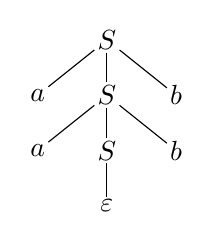
\begin{tikzpicture}[level distance=20pt, sibling distance=25pt, every node/.style={inner sep=1pt}]
\node {$S$}
  child {node {$a$}}
  child {node {$S$}
    child {node {$a$}}
    child {node {$S$} child {node {$\varepsilon$}} }
    child {node {$b$}}
  }
  child {node {$b$}};
\end{tikzpicture}
\vspace{-4pt}
\end{center}
\hrule
\textbf{Ambiguity Resolution for} $G: A \to -A \mid A-\text{id} \mid \text{id}$. Parse trees for \texttt{-id-id}:\\[2pt]
\noindent\begin{minipage}[t]{0.495\textwidth}
\textbf{Infix priority ($G_i$):} $-(\text{id}-\text{id})$\\
$G_i: A \to C \mid -A$\\
$\phantom{G_i: } C \to \text{id} \mid C - \text{id}$
\vspace{-4pt}
\begin{center}
\begin{tabular}{cc}
\textbf{Ambiguous} & \textbf{Solution (}$G_i$\textbf{)} \\
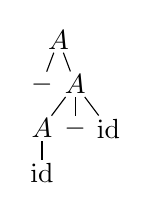
\begin{tikzpicture}[level distance=16pt, sibling distance=12pt, every node/.style={inner sep=1pt}]
\node {$A$}
  child {node {$-$}}
  child {node {$A$}
    child {node {$A$} child {node {$\text{id}$}}}
    child {node {$-$}}
    child {node {$\text{id}$}}
  };
\end{tikzpicture}
&
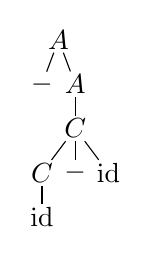
\begin{tikzpicture}[level distance=16pt, sibling distance=12pt, every node/.style={inner sep=1pt}]
\node {$A$}
  child {node {$-$}}
  child {node {$A$}
    child {node {$C$}
      child {node {$C$} child {node {$\text{id}$}}}
      child {node {$-$}}
      child {node {$\text{id}$}}
    }
  };
\end{tikzpicture}
\end{tabular}
\vspace{-4pt}
\end{center}
\end{minipage}%
\hfill
\begin{minipage}[t]{0.495\textwidth}
\textbf{Prefix priority ($G_p$):} $(-\text{id})-\text{id}$\\
$G_p: A \to B \mid A - \text{id}$\\
$\phantom{G_p: } B \to -B \mid \text{id}$
\vspace{-4pt}
\begin{center}
\begin{tabular}{cc}
\textbf{Ambiguous} & \textbf{Solution (}$G_p$\textbf{)} \\
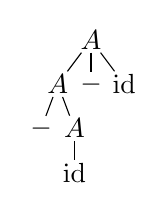
\begin{tikzpicture}[level distance=16pt, sibling distance=12pt, every node/.style={inner sep=1pt}]
\node {$A$}
  child {node {$A$}
    child {node {$-$}}
    child {node {$A$} child {node {$\text{id}$}}}
  }
  child {node {$-$}}
  child {node {$\text{id}$}};
\end{tikzpicture}
&
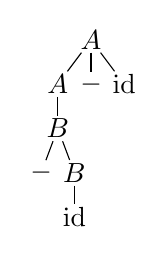
\begin{tikzpicture}[level distance=16pt, sibling distance=12pt, every node/.style={inner sep=1pt}]
\node {$A$}
  child {node {$A$}
    child {node {$B$}
      child {node {$-$}}
      child {node {$B$} child {node {$\text{id}$}}}
    }
  }
  child {node {$-$}}
  child {node {$\text{id}$}};
\end{tikzpicture}
\end{tabular}
\end{center}
\end{minipage}\\
$L(G) = L(-^*\text{id}(-\text{id})^*)$
\hrule
\textbf{Divisibility check.}\\
For binary string $(b_k b_{k-1}\dots b_0)$, to check divisibility by integer $n$:\\
1. Initialize $r=0$ \quad 2. Scan bits from left to right, updating $r \leftarrow (2r + b_i)\bmod n$\\
After the last bit:\\
- if (r=0), the binary number is divisible by (n)\\
- otherwise, it is not\\
\textbf{Special case.} if $(n=2^m)$, just check whether the last (m) bits are all (0).\\
\begin{minipage}[t]{0.495\textwidth}
\textbf{$L_1$: binary strings divisible by 3}, NFA:\\
After init state, state is $q_k$ represents $r = k$
\begin{center}
\begin{tabular}{c|cc}
\toprule
State & $0$ & $1$ \\
\midrule
$q_{\mathit{init}}$ & $q_0$ & $q_1$ \\
\accept{q_0}        & $q_0$ & $q_1$ \\
$q_1$               & $q_2$ & $q_0$ \\
$q_2$               & $q_1$ & $q_2$ \\
\bottomrule
\end{tabular}
\end{center}
\end{minipage}
\begin{minipage}[t]{0.495\textwidth}
\textbf{2. binary strings divisible by 4}, NFA:
\begin{center}
\begin{tabular}{c|cc}
\toprule
State & $0$ & $1$ \\
\midrule
$q_{\mathit{init}}$ & $q_0$ & $q_1$ \\
\accept{q_0}        & $q_0$ & $q_1$ \\
$q_1$               & $q_2$ & $q_3$ \\
$q_2$               & $q_0$ & $q_1$ \\
$q_3$               & $q_2$ & $q_3$ \\
\bottomrule
\end{tabular}
\end{center}
\end{minipage}\\
\textit{Example.}\; $e_2 = [+\!\mid\!-]?\Big(\big([0\text{-}9]^+(.[0\text{-}9]^*)?\;\big|\;.[0\text{-}9]^+\big)\big([eE][+\!\mid\!-]?[0\text{-}9]^+\big)?\Big)$\\[4pt]
Inside-out:
\[
\begin{aligned}
A &= [+\!\mid\!-]? &&\to \text{true} \quad\text{(optional)}\\
B &= [0\text{-}9]^+ &&\to \text{false} \quad\text{(one-or-more, base not nullable)}\\
C &= (.[0\text{-}9]^*)? &&\to \text{true} \quad\text{(optional)}\\
D &= .[0\text{-}9]^+ &&\to \text{false} \land \text{false} = \text{false}\\
BC\mid D &: \;(\text{false}\land\text{true})\lor\text{false} &&= \text{false}\\
E &= ([eE][+\!\mid\!-]?[0\text{-}9]^+)? &&\to \text{true} \quad\text{(optional)}\\
\text{body} &= (BC\mid D)\cdot E &&= \text{false}\land\text{true} = \text{false}\\[2pt]
\text{nullable}(e_2) &= A \land \text{body} &&= \text{true}\land\text{false} = \boxed{\textbf{false}}
\end{aligned}
\]
\end{minipage}
\end{document}


